Since the 1970s \parencite{article14}, the decade in which the microprocessor era started, the overall performance of a processor has increased \parencite{inproceedings4}. This goal was achieved by several points, including ``\textit{sophisticated process technology, innovative architecture or micro-architecture}'' \parencite[see][Chapter 1, p2]{inproceedings4}. In fact, increasing the clock speed of a single core processor, like Moore's Law predicted \parencite{article14}, was usually reached by increasing the number of transistors on the chip \parencite{article14}. However, this go along side with the increase in complexity \parencite[see][Pollack’s rule]{article14}, which mean, that doubling the logic of a processor result in a performance boost of only 40\% \parencite[see][Chapter 2]{article14}.

Another huge problem chip manufacturers have to deal with is leakage power \parencite[see][Chapter 2, p3]{inproceedings4}, because the ``\textit{transistor leakage current increases as the chip size shrinks}'' \parencite[see][p2]{article14} [see Chart \ref{fig:leackagePer}]. An increase of leakage current of the transistors also result in a increase of the die's temperature \parencite{inproceedings4} along side the total power consumption as well.
\begin{figure}[h!]
	\centering
	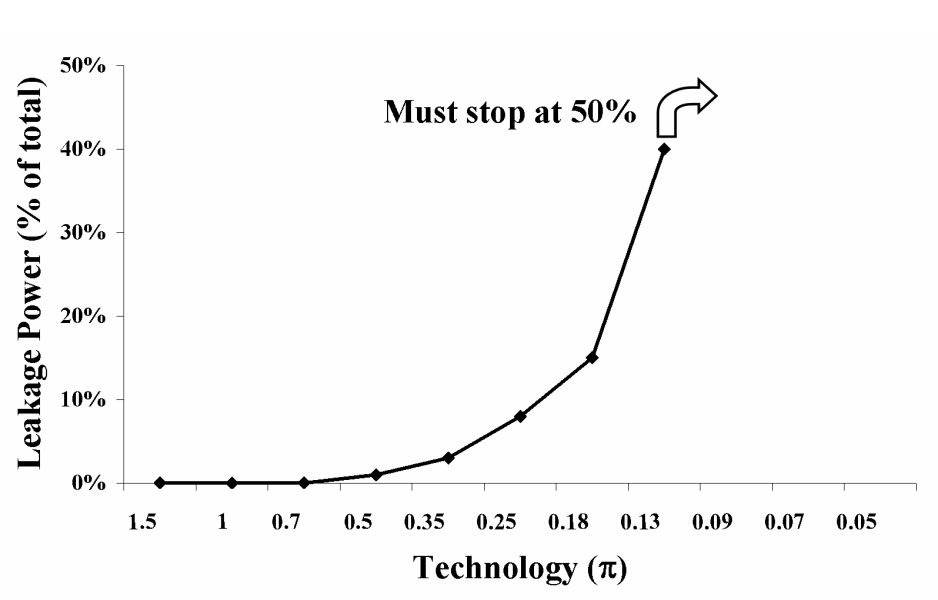
\includegraphics[scale=0.25]{leackage-power_vs_process-technology.png}
	\caption{
		Leakage Power (\% of total) vs. process technology \parencite{inproceedings4}
	}
	\label{fig:leackagePer}
\end{figure}

Furthermore, a increase of the processor clock frequency to speed up the performance is only available to a suffisticating limit of 4GHz \parencite{article14}. After this frequency threshold, also known as reaching the power wall, the ``\textit{power dissipation}'' \parencite[see][p2]{article14} increases again.

Facing these types of problems such as ``\textit{chip fabrication costs, fault tolerance, power efficiency, heat dissipation}'' \parencite[see][p3]{article14} along side with increasing processor performance, the only possible solution chip manufacturers and companies could offer was parallelism. 

\newpage

\section{Basic Concept}

Parallelism for processing is not something new. But due to the fact that real thread level parallelism [see Chapter \ref{subchap:threadLevelParallelism}] was only available after dual or multi-core processors were invented in 2005 \parencite{internet6}, the topic itself and efficient software implementations are still treated in scientific work \parencite{book3} \parencite{article2}.

\begin{figure}[h!]
	\centering
	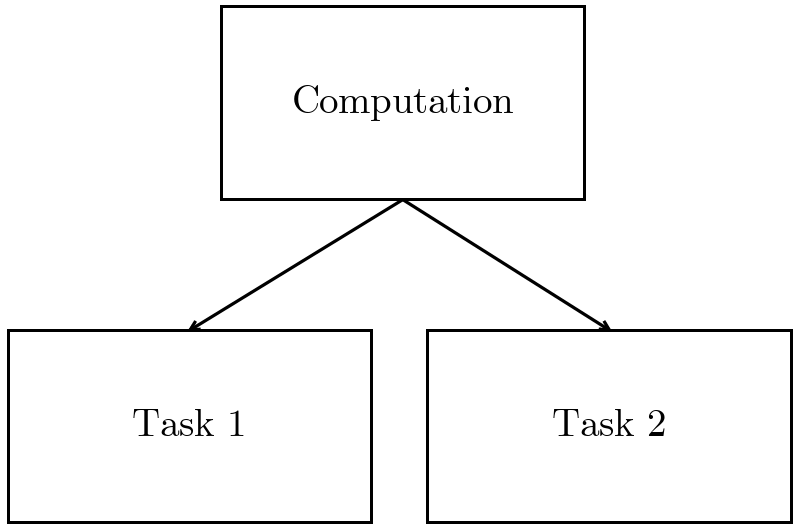
\includegraphics[scale=0.3]{basic-parallelism.png}
	\caption{
		The basic concept of a simple concurrency computation.
	}
	\label{fig:basicPara}
\end{figure}

In general, parallelism for programming means to split up a task or a computation into several sub tasks [e.g. Figure \ref{fig:basicPara}] or results, to decrease the execution time. Depending on the problem itself, these separated tasks can be independent or connected [see Chapter \ref{chap:parallelPrinciples}]. If we want to talk about the general concept of parallelism, we have to take a closer look to some mathematical laws, which try to describe the availability to parallel task execution and their limits.

\subsection{Amdahl's Law}

The first one, which quantifies parallelism, is called Amdahl's Law \parencite{inbook1}. During the publication period of Amdahl's paper \parencite{book6}, critics claimed ``\textit{that the organization of a single computer has reached its limits and that
truly significant advances can be made only by interconnection of a multiplicity of computers}” \parencite[see][p80]{inbook1}. Of course this can be transferred on single and multi-core processors or even on multi threading \parencite[see][Chapter 1.3, p2]{phdthesis1}, but in fact, like Amdahl claimed too, addressing hardware \parencite{inbook1}, and nowadays switching context time was not considered in this case.

Amdahl's Law wants ``\textit{to provide an upper limit on speedup}'' \parencite[see][p81]{inbook1} in general to point out that there is a overhead \parencite{inbook1}, which can not pe implemented in parallel, but at the same time, ``\textit{apart from the sequential fraction, the remaining computations are perfectly parallelizable}'' \parencite[see][p81]{inbook1}.

\newpage

\begin{figure}[h!]
	\centering
	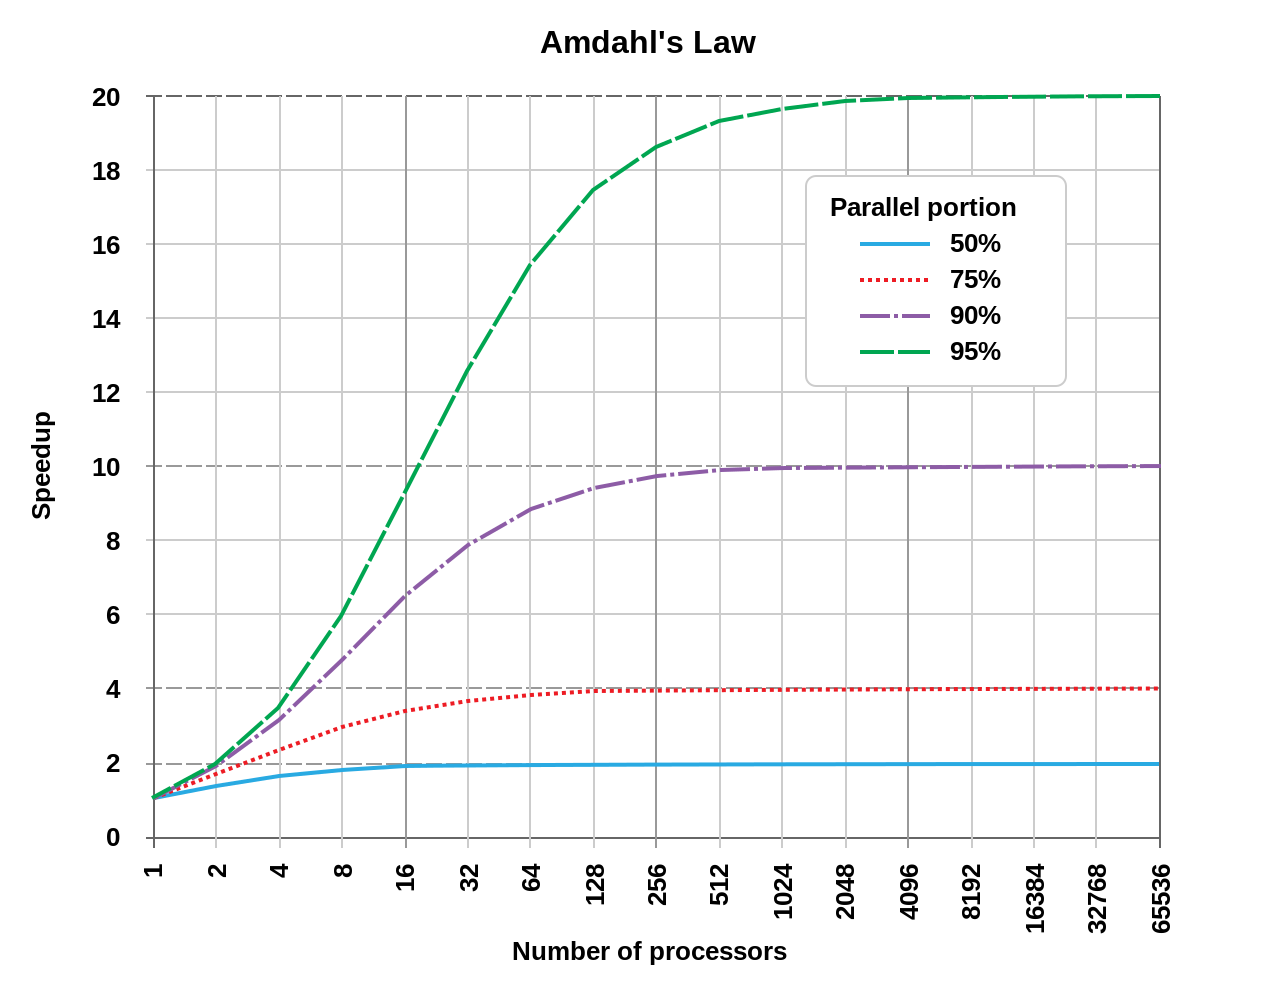
\includegraphics[scale=0.95]{amdahls-law.png}
	\caption{
		The limited speed-up of a program, which can be parallelized, depending on the number of parallel executions \parencite{image1} \parencite[similar to][p4]{phdthesis1}.
	}
	\label{fig:admLaw}
\end{figure}

\noindent So regarding to Amdahl's Law, there has to be an upper limit of parallelism, due to the fact, that some sequential fractions still exists. In order to be able to describe this relationship, the time required to perform a calculation at once is related to the total time in parallel execution:

``\textit{Let t\textsubscript{1} be the time taken by one processor solving a computational problem and t\textsubscript{p} be the time taken by p processors solving the same problem. Finally let us denote the supposed inherently sequential fraction of instructions by f. Then, according to Amdahl, t\textsubscript{p} = t\textsubscript{1}(f+(1-f)/p) and the speedup obtainable by p processors can be expressed as}'' \parencite[see][p81]{inbook1}:

\begin{equation} \label{formula:amd}
	s = \frac{t_1}{t_p} = \frac{1}{f + (1 - f) / p}
\end{equation}
\\[2pt]
For example, a program which contains 90\% of parallelizable code [see Figure \ref{fig:admLaw}] reaches his speed up limit at around 512 cores [formula  \ref{formula:amdLimes}]; in this case we substitute f= 0.2/2. After that number of processor cores, an significant speed up increase is not noticeable anymore . 

\begin{equation} \label{formula:amdLimes}
	\lim_{p \to \infty f \to 0.1} \left( \frac{t_1}{t_p} \right) = \lim_{p \to \infty} \left( \frac{1}{0.1 + (1 - 0.1) / p} \right) = 10
\end{equation}
\\[2pt]
Many other authors tried to claim that this upper limit of speed up, both in theory and practice, is not the final end. To proof that, only to mention a few , they took into account the ``\textit{energy per instruction (EPI)}" \parencite[Annavaram et al. in][Chapter 3,  p81]{inbook1}, a case study depending on ``\textit{asymmetric (or heterogeneous) chip multiprocessor architectures}'' \parencite[Kumar et al. in][Chapter 3,  p81]{inbook1} or even considering ``\textit{disk arrays to reduce input-output requirements}'' \parencite[Patterson et al. in][Chapter 3,  p81]{inbook1}.

\newpage

\subsection{Gustafson’s Law's}

Due to the fact that Gustafson’s Law's is based on ``the same concepts as the
bases of Amdahl’s law, it is more a variant, rather than a refutation'' \parencite[see][p81]{inbook1}. But in fact, it is another mathematical consideration, which offers, in comparison to Amdahl's Law, no upper speed up limit regarding parallelism. Related to Gustafson, the time a single core processor needs solving the same computational problem on the sequential would be \textit{ft\textsubscript{p}}, and on the parallelizable part \textit{(1-f)pt\textsubscript{p}}. Therefore, the total amount of achievable speed up by p processors can thus be calculated

\begin{equation} \label{formula:gustLaw}
	s = \frac{t_1}{t_p} = \frac{ft_p + (1 - f)pt_p}{t_p} = f + (1 - f)p
\end{equation}
\\[2pt]
using the formula \ref{formula:gustLaw} above. In this case, ``f is the same “inherently sequential” fraction of instructions as in the case of Amdahl’s law'' \parencite[see][p81]{inbook1}. In addition to that, he doesn't take the ``sequential input-output requirements proportional to input and output sizes into account'' \parencite[see][p81]{inbook1}.

\begin{figure}[h!]
	\centering
	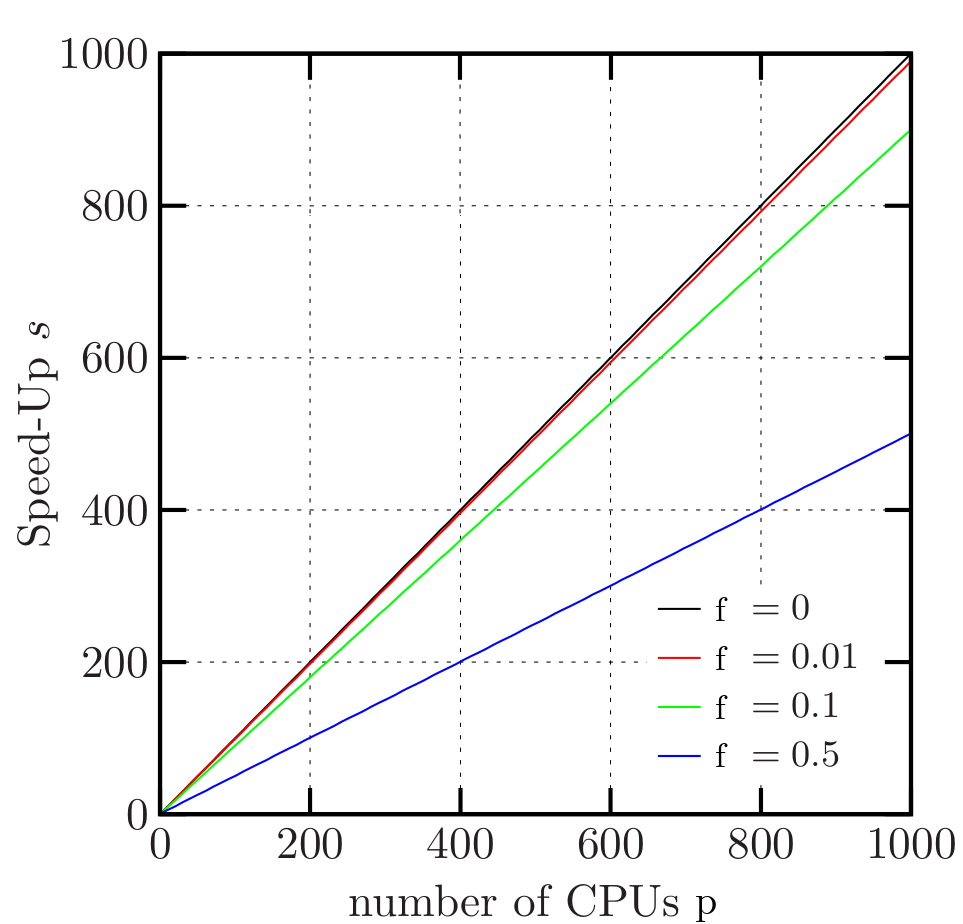
\includegraphics[scale=0.28]{gustafssons-law.png}
	\caption{
		Gustafson’s Law. In contrast to Amdahl we now have no upper limit to the speed up. \textit{f} only determines the slope of the speed-up \parencite{article19}.
	}
	\label{fig:gustLaw}
\end{figure}

Regarding to \parencite{inbook1}, neither Amdahl's or Gustafson’s Law are suitable to quantify parallelism in theory and practice, because both don't take into account, that ``sequential fractions of computations have negligible effect on speedup if the growth rate of the parallelizable fraction is higher than that of the sequential fraction.'' \parencite[see][Chapter 7, p88]{inbook1}.

Furthermore, \parencite{inbook1} point out, that no simple formula governing parallelism exists. Both laws are more of an attempt to describe experimental results, and therefore understood rather as a draft rule of thumb as a law.

\newpage

\subsection{Concurrency in general} \label{chap:concurrGeneral}

\begin{itemize}
	\item ...\parencite[see][p3]{internet1}
	\item ...\parencite[see][p3]{internet2}
	\item ...
\end{itemize}

\newpage

\subsection{Principles of Parallel Computing}\label{chap:parallelPrinciples}

\textbf{Emphasises design}:
Amdahl's law highlights the pitfalls of looking for
sticking-plaster speed-ups in serial programs –
design for concurrency \parencite[see][p4]{article6}
\\\\\textbf{Aim of concurrency and their effects} on program structure or implementation \parencite[see][p5]{article6}:
\begin{itemize}
  \item \underline{Flexibility}: Environments will be more heterogeneous.
  \item \underline{Efficiency}:	parallel for a speed-up purposes, more pitfalls (memory latency, thread overheads etc.)
  \item \underline{Simplicity}:	Parallel codes will be more complicated. All the more reason to strive for maintainable, understandable programs.\\
\end{itemize}
...\parencite[see][p11 ff.]{article6}

\newpage

\section{Definition of parallel mathematical computations}

\underline{Mathematical examples} \parencite{inbook1}:
\begin{itemize}
	\item ...\parencite[see][p8]{internet1}
	\item ...\parencite[see][p4]{internet2}
	\item ...\parencite[see][p398]{article7}
\end{itemize}

\newpage

\section{Parallel Computer Architecture}
The terminology of computer architecture was invented in 1960s by the designers of IBM System to describe the structure of a computer. Computer architect’s task is to write an suitable program code for the machine,keeping in mind everytime this structure of computer, understanding all the factors like state-of-the-art technologies at each design level and changing those designs tradeoffs for their specific applications.\
Parallel computing means the situation where tasks are separated into discrete parts that can be executed concurrently. Each part is diffused into a larger series of instructions which will be executed simultaneously on different CPUs. These kind of parallel systems have to deal with the simultaneous use of multiple computer resources that can can include either a single computer with multiple CPUs, ori a number of computers connected by a network creating a parallel processing cluster or combination of both.\
The crux of parallel processing are CPUs. Based on the number of instruction and data streams that can be processed simultaneously, computing systems are classified into four major categories based on Flynn’s Taxonomy.
\\
...\parencite[see][p9]{book1} \\
...examples of parallelism \parencite[see][p11]{book1} \\
...links 1) \\
...\parencite[see][p9 ff.]{book5}


\subsection{Flynn's Taxonomy of Parallel Architectures}
Flynn’s classification was first elaborated and proposed by Michael Flynn in 1966 and represents a scheme which is based on the notion of information stream. The term ‘stream’ defines a sequence or flow of either one of both existent types of information which flows and are operated into a processor: instructions or data. Instruction stream defines the sequence of instructions performed by CPU, as in the same time the data stream defines the data traffic exchanged between the memory and CPU.His taxonomy left aside the machine’s structure for classification of parallel computers and took over a whole new concept focusing on multiplicity of instructions and data streams observed by the CPU during the execution.\
(IDK HOW TO MAKE A LIST)The major four categories are the followings:
SISD (single-instruction,single-data) systems
It designs an sequential computer which exploits no parallelism in either the instruction stream nor data stream.  An SISD computing system  is a uniprocessor machine capable of single stream executions.
SIMD(single-instruction, multiple-data) systems
It designs a multiprocessor machine capable of executing a single instruction stream on multiple different data streams. Instructions can be executed sequentially, such as by pipelining,  or in parallel by multiple functional units.
MISD (multiple instruction streams, single data stream) systems
It designs a multiprocessor machine capable of executing different instructions streams on the same data stream.  
MIMD (multiple instruction streams, multiple data streams) 
It designs a multiprocessor machine capable of executing multiple instructions streams on multiple data streams. This architectures include multi-core superscalar processors and distributed systems. 
\\
...\parencite[see][p5]{internet1}\\
...\parencite[see][p13]{book1}\\
...\parencite[see][p4]{book5}\\
...\parencite[see][p2]{book6}\\
...\parencite[see][p15-p26]{internet2}

\subsection{Thread Level Parallelism}\label{subchap:threadLevelParallelism}

...\parencite[see][p24]{book1}\\
...\parencite[see][p14]{article6}

\section{Parallel Programming Models}

\textbf{Steps to evaluate a proper parallel design} \parencite[see][p6]{article6}:
\begin{enumerate}
	\item Finding Concurrency
	\item Algorithm Structure
	\item Supporting Structures
	\item Implementation Mechanisms
\end{enumerate}

\newpage

\subsection{Classification of Parallel Programming Models}

\subsubsection{Process Interaction}

...\parencite[see][p4]{internet1}

\subsubsection{Problem decomposition}

...\parencite[see][p105 ff.]{book1}